
%\subsection{3D Enviroment Specifics}
\section{Implementation and Results}

The simulation follow the ray tracing technique outlined by
\citet{bell1997simulation} for side scan sonar, but applies it to a forward
looking sonar imaging sonar (section \ref{ss:avaible_models}). It also uses a
noising adding step as suggested by \citet{coiras2009gpu} with statistics
provided by \citet{maussang2007mean}.
No movement induced distortion was considered, some approachs to add this
feature is available on \citet{bell1999techniques,borawski2005sonar}.

Sonar parameters follow a Tritech's Micron sonar\cite{micronsonar}
information as output power, dynamic gain, beam step and sensibility were found
on official Tritech's documentation\cite{micronsonar,micronmodem}. The directional
gain was measured by the National Physical Laboratory, UK.

Simulation's output is, just as on the sonar, a sequence of arrays with values
between 0 and 255. Each element of the sequence is a bearing, direction of the
emitted sound pulse, and the array's components are the bins' values, sound
intensity received at some range of distances (calculated from echo delay).

\begin{figure}[h]
	\centering
	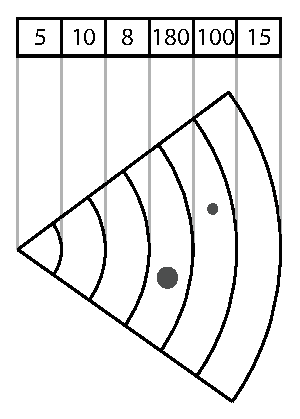
\includegraphics[scale=1.,clip]{Chap2/fig/sonarresponse.eps}
	\caption{Exemple of an array for a bearing direction. Actual arrays are
	longer, depending on resolution.}
	\label{fig:bins}
\end{figure}

The algorithm implementation uses the programming language Python with the
mathematical library NumPy, specially for efficient linear algebra. Most of the
treatment uses linear algebra to treat batch of rays at once.
\begin{algorithm}
\caption{ANO AGL}
\begin{algorithmic}
\Require BeamDirections
\ForAll{$\theta_i \in$ BeamDirections}
\If {$i\geq maxval$}
    \State $i\gets 0$
\EndIf
\EndFor
\end{algorithmic}
\end{algorithm}